% Presentatie Project 7 (tussentijds)
\documentclass{beamer}

\mode<presentation>

\usepackage[dutch]{babel}
%\usepackage{beamerthemesplit}
\usetheme{Berlin}
\useinnertheme{rounded}
\usecolortheme{rose}
\setbeamertemplate{navigation symbols}{} 

\title{Hogeschool Rotterdam}
\author{Sebastiaan Polderman \and\\ Paul Sohier \and\\ Rudolf Koster \and\\ Tristan Hakkaart}
\date{\today}

\begin{document}

\frame{
  \titlepage
} 

\frame{
  \frametitle{Inhoud}
  \tableofcontents
}

 \section{Introductie}
 \frame{
   \frametitle{Wie zijn wij en wat doen we hier?}
   \begin{itemize}
    \item<1-> Hogeschool Rotterdam
    \item<2-> Sebastiaan Polderman
    \item<2-> Paul Sohier
    \item<2-> Rudolf Koster
    \item<2-> Tristan Hakkaart
   \end{itemize}
 }

\section{HRO}
\frame{
  \frametitle{Over Hogeschool Rotterdam}
  \begin{itemize}
    \item<1-> 80 Opleidingen
    \item<2-> 28500 studenten
    \item<3-> 8 Locaties
  \end{itemize}
}

\section{CMI}
\frame{
  \frametitle{CMI}
  \begin{itemize}
    \item<1-> 9 Opleidingen
    \item<2-> 2000 studenten
    \item<3-> 2 Locaties
  \end{itemize}
}

\section{Technische Informatica}
\frame{
  \frametitle{Technische Informatica}
  \begin{itemize}
    \item<1-> Wat doen we op school
    \item<2-> Waarom bij elektro presenteren?
    \item<3-> Wat is er dan zo speciaal aan?
  \end{itemize}
}

\section{Projecten}
\frame{
  \frametitle{Projecten}
  \begin{itemize}
    \item<1-> Fluffy
    \item<2-> 3D Printer
    \item<3-> Andere projecten
  \end{itemize}
  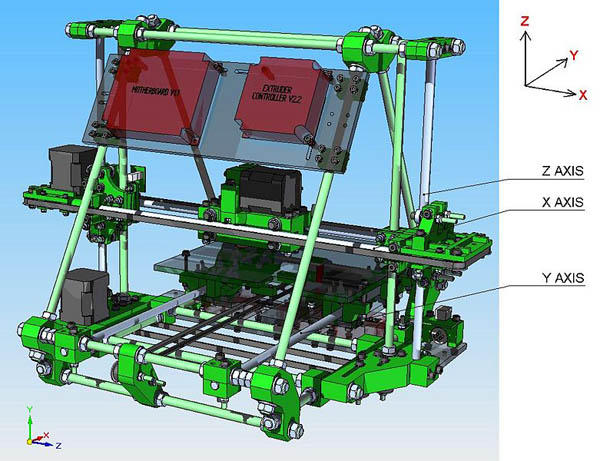
\includegraphics[scale=0.4]{Mendel_GA.jpg}
}

\section{Project RepRap}
\frame{
  \frametitle{RepRap, wat is het?}
  \begin{itemize}
    \item<1-> Open source 3D printer
    \item<1-> Combinatie tussen elektronica en technische informatica
    \item<2-> Project zelf bedacht, geen standaard project
  \end{itemize}
  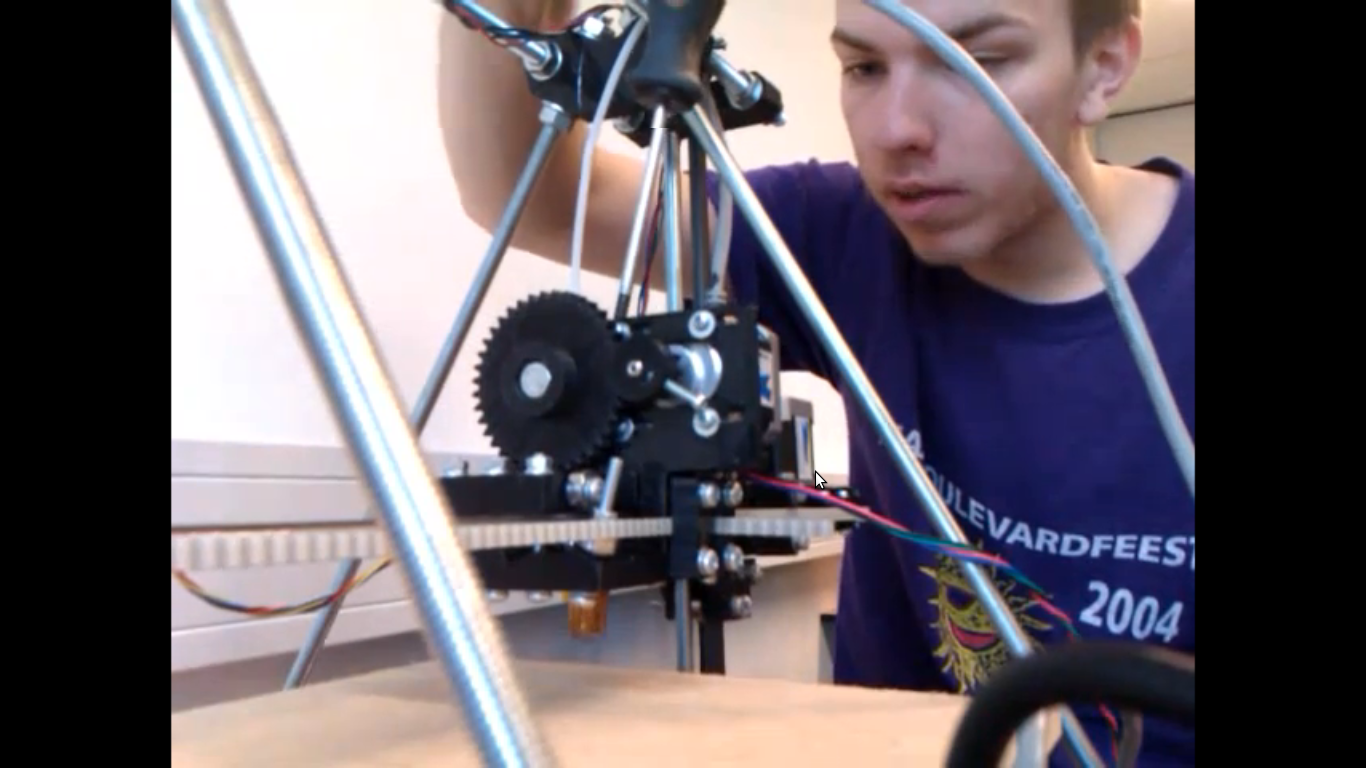
\includegraphics[scale=0.2]{Schermafdruk-1.png}
}

\frame{
  \includegraphics[scale=0.085]{IMG_0953_bwt.jpg}
}
\frame{
  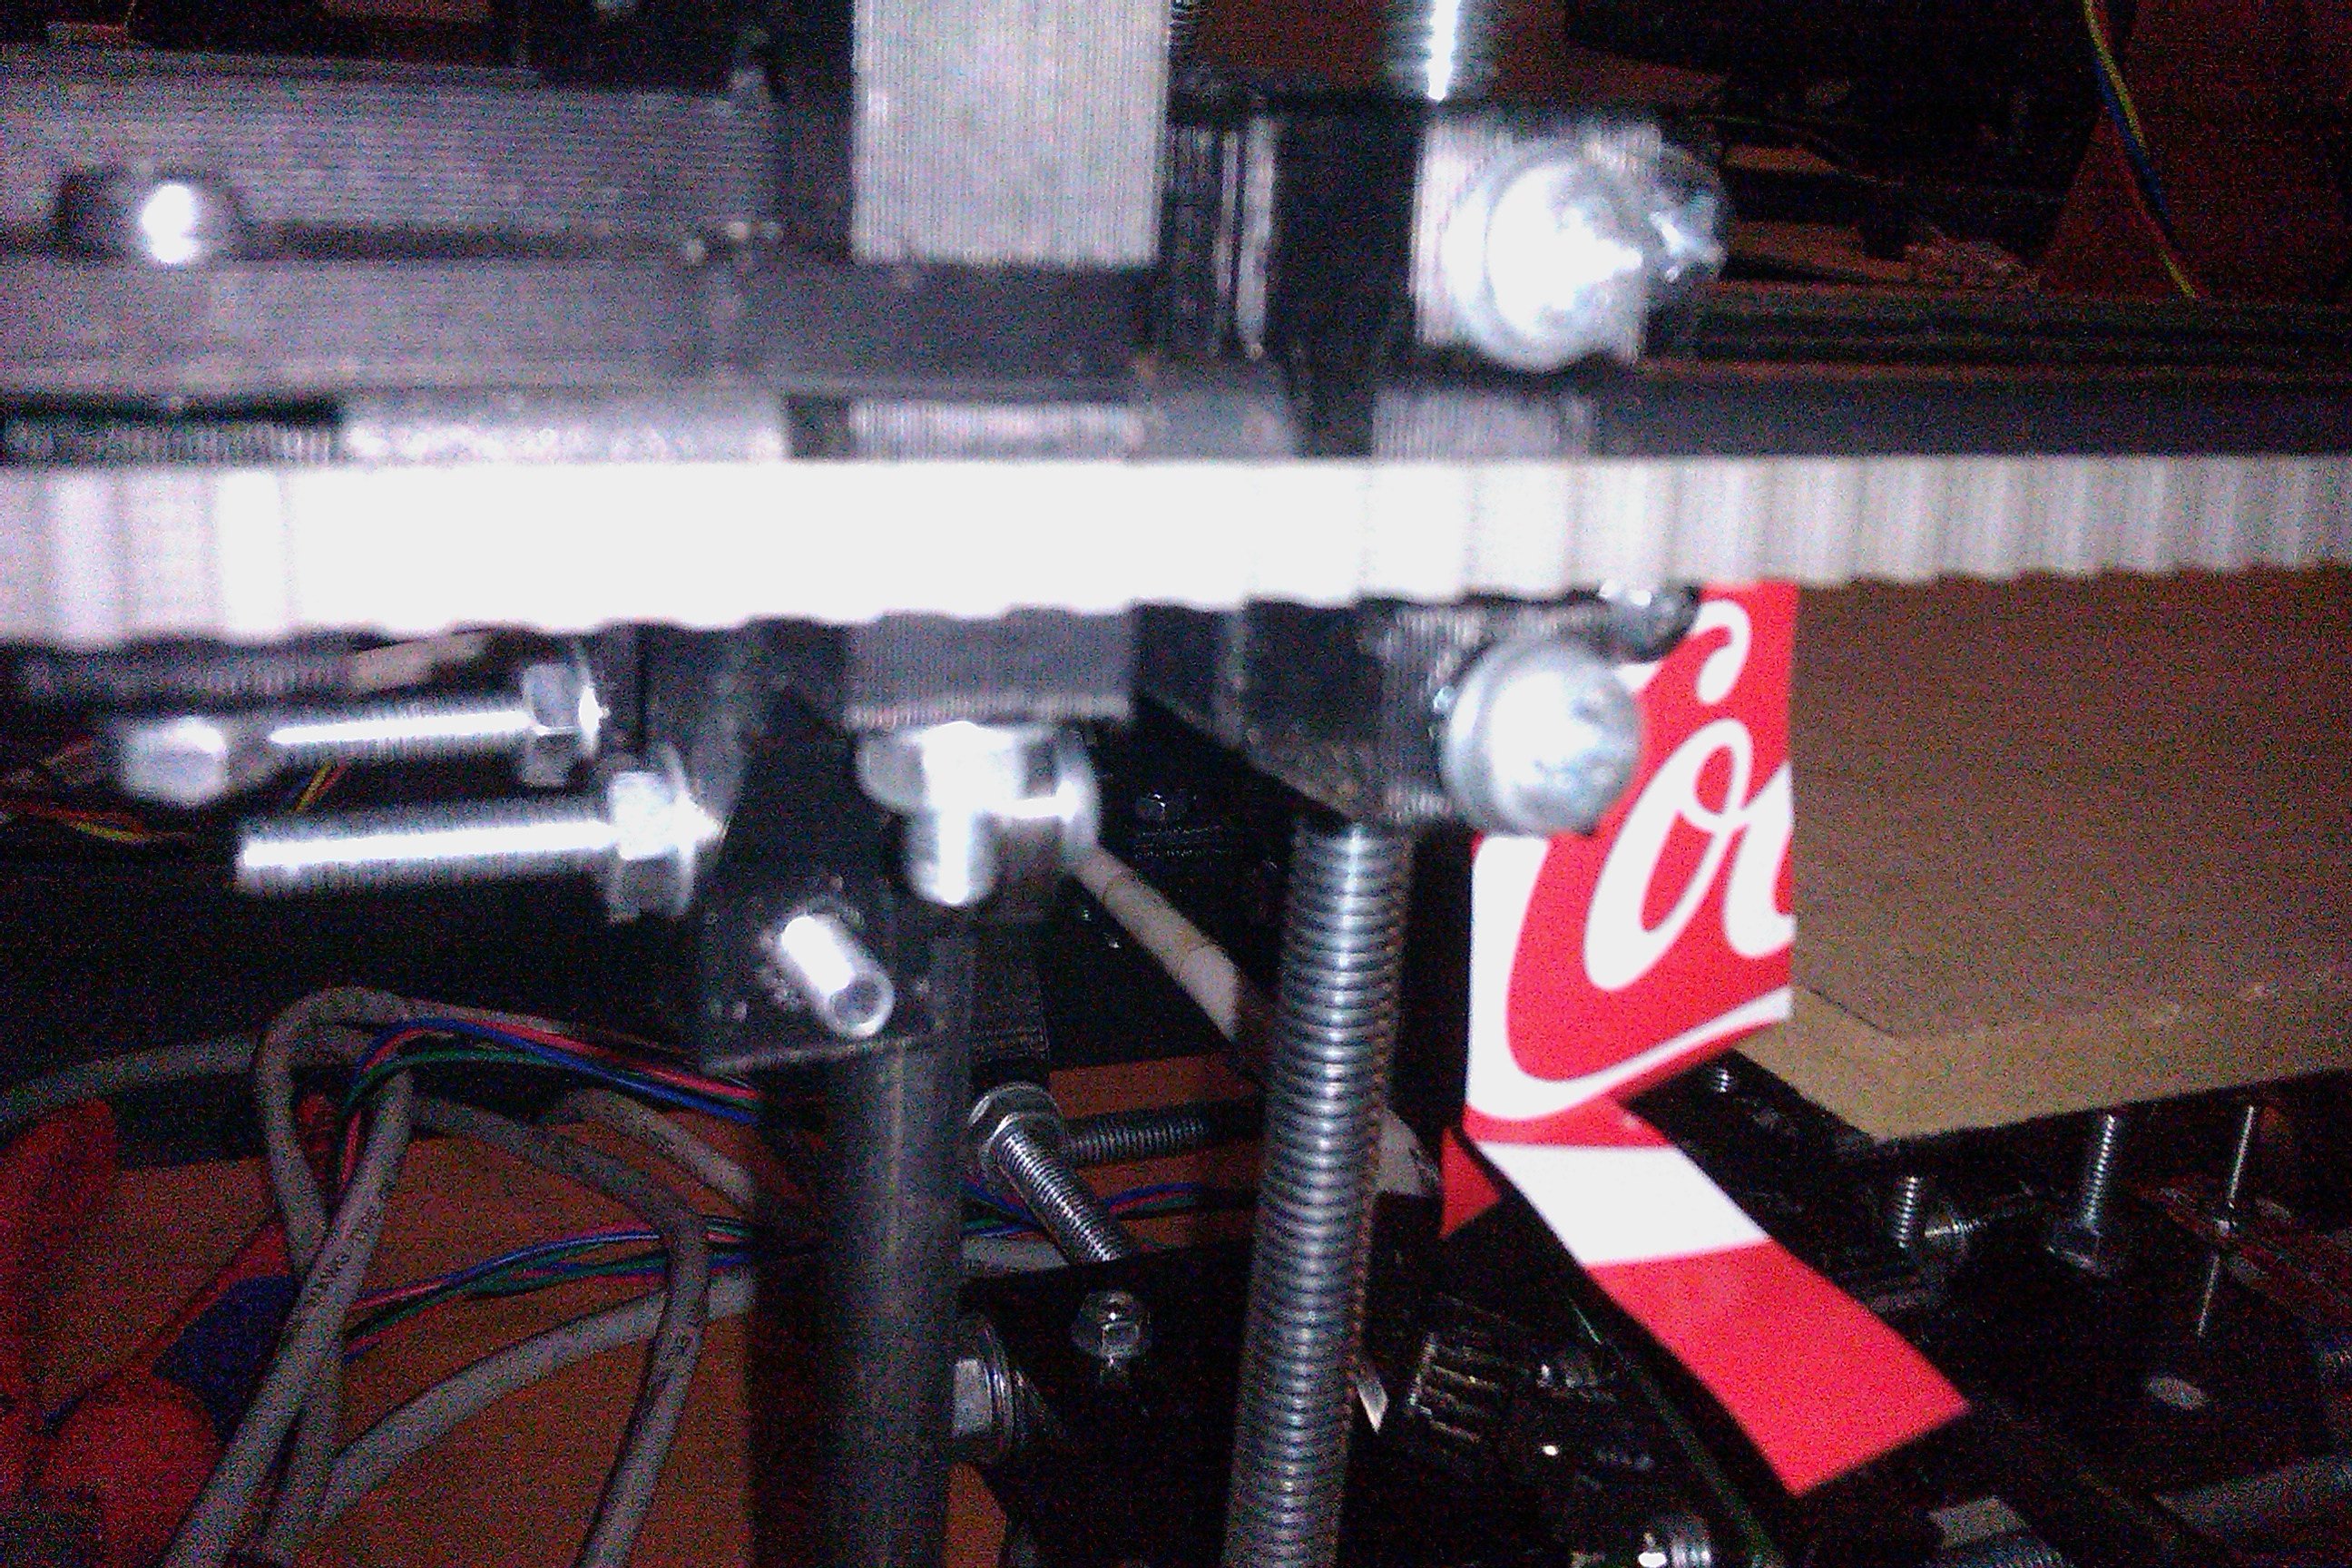
\includegraphics[scale=0.125]{imag0366.jpg}
}
\frame{
  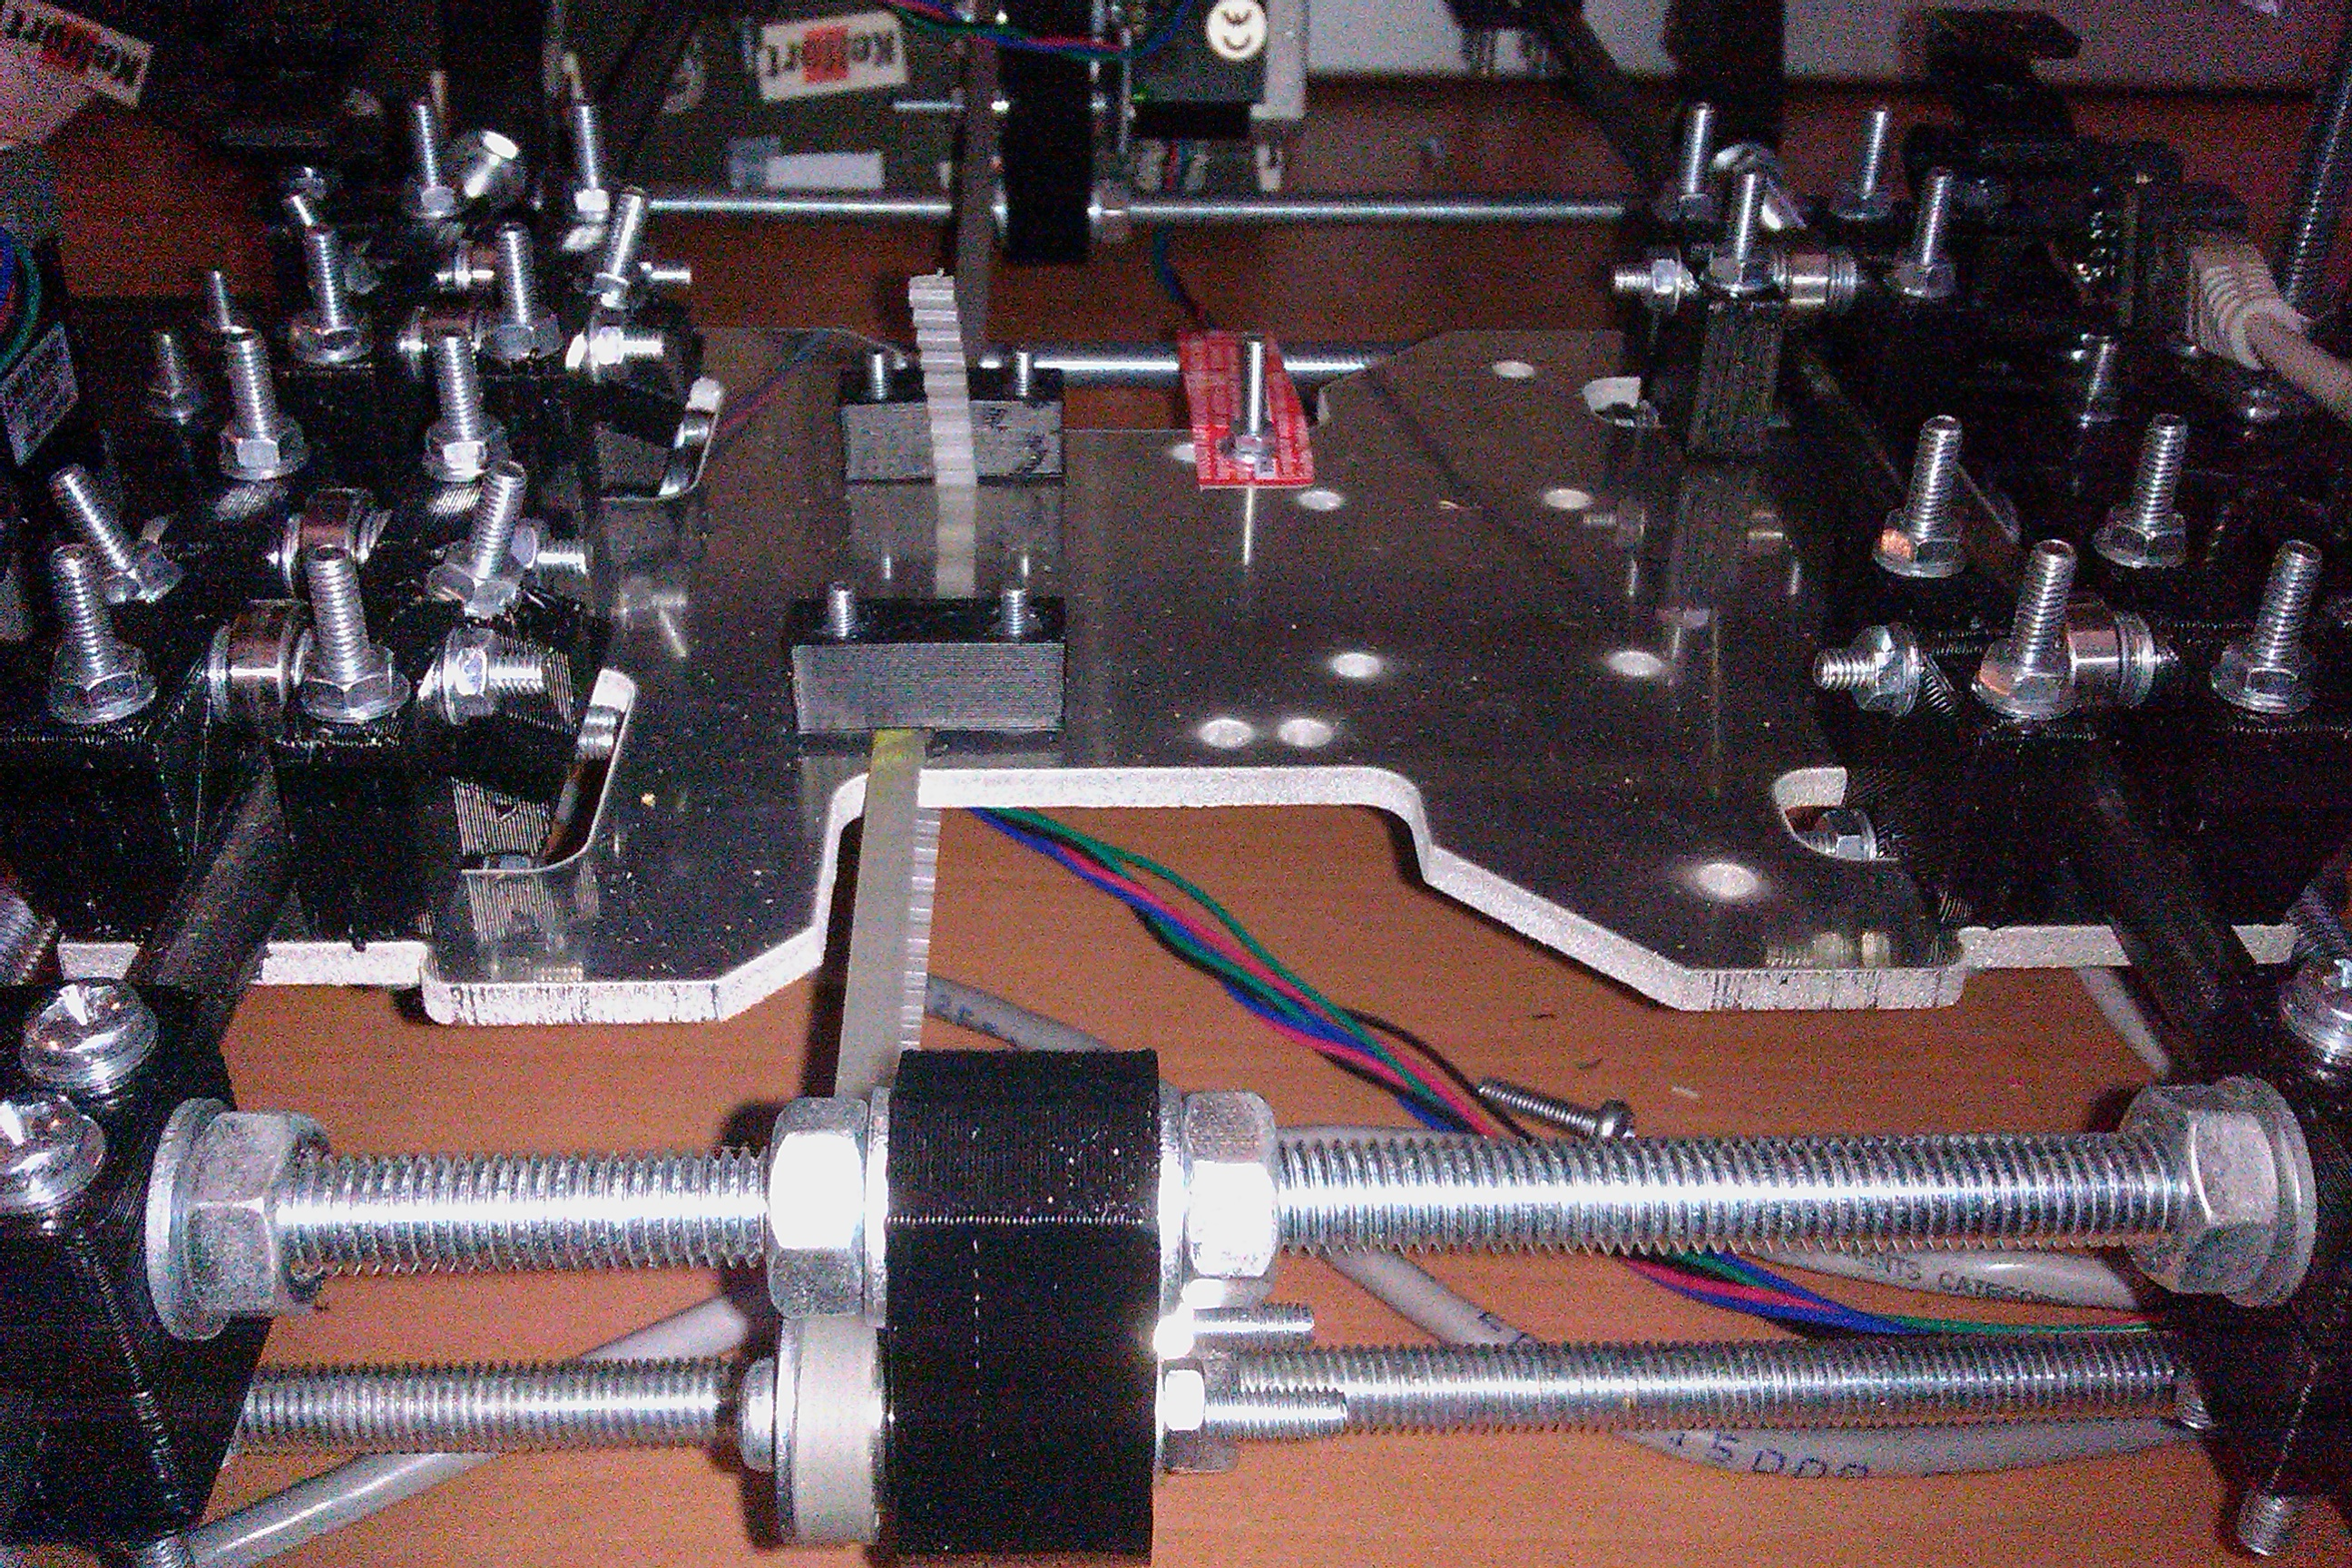
\includegraphics[scale=0.125]{imag0363.jpg}
}
\frame{
  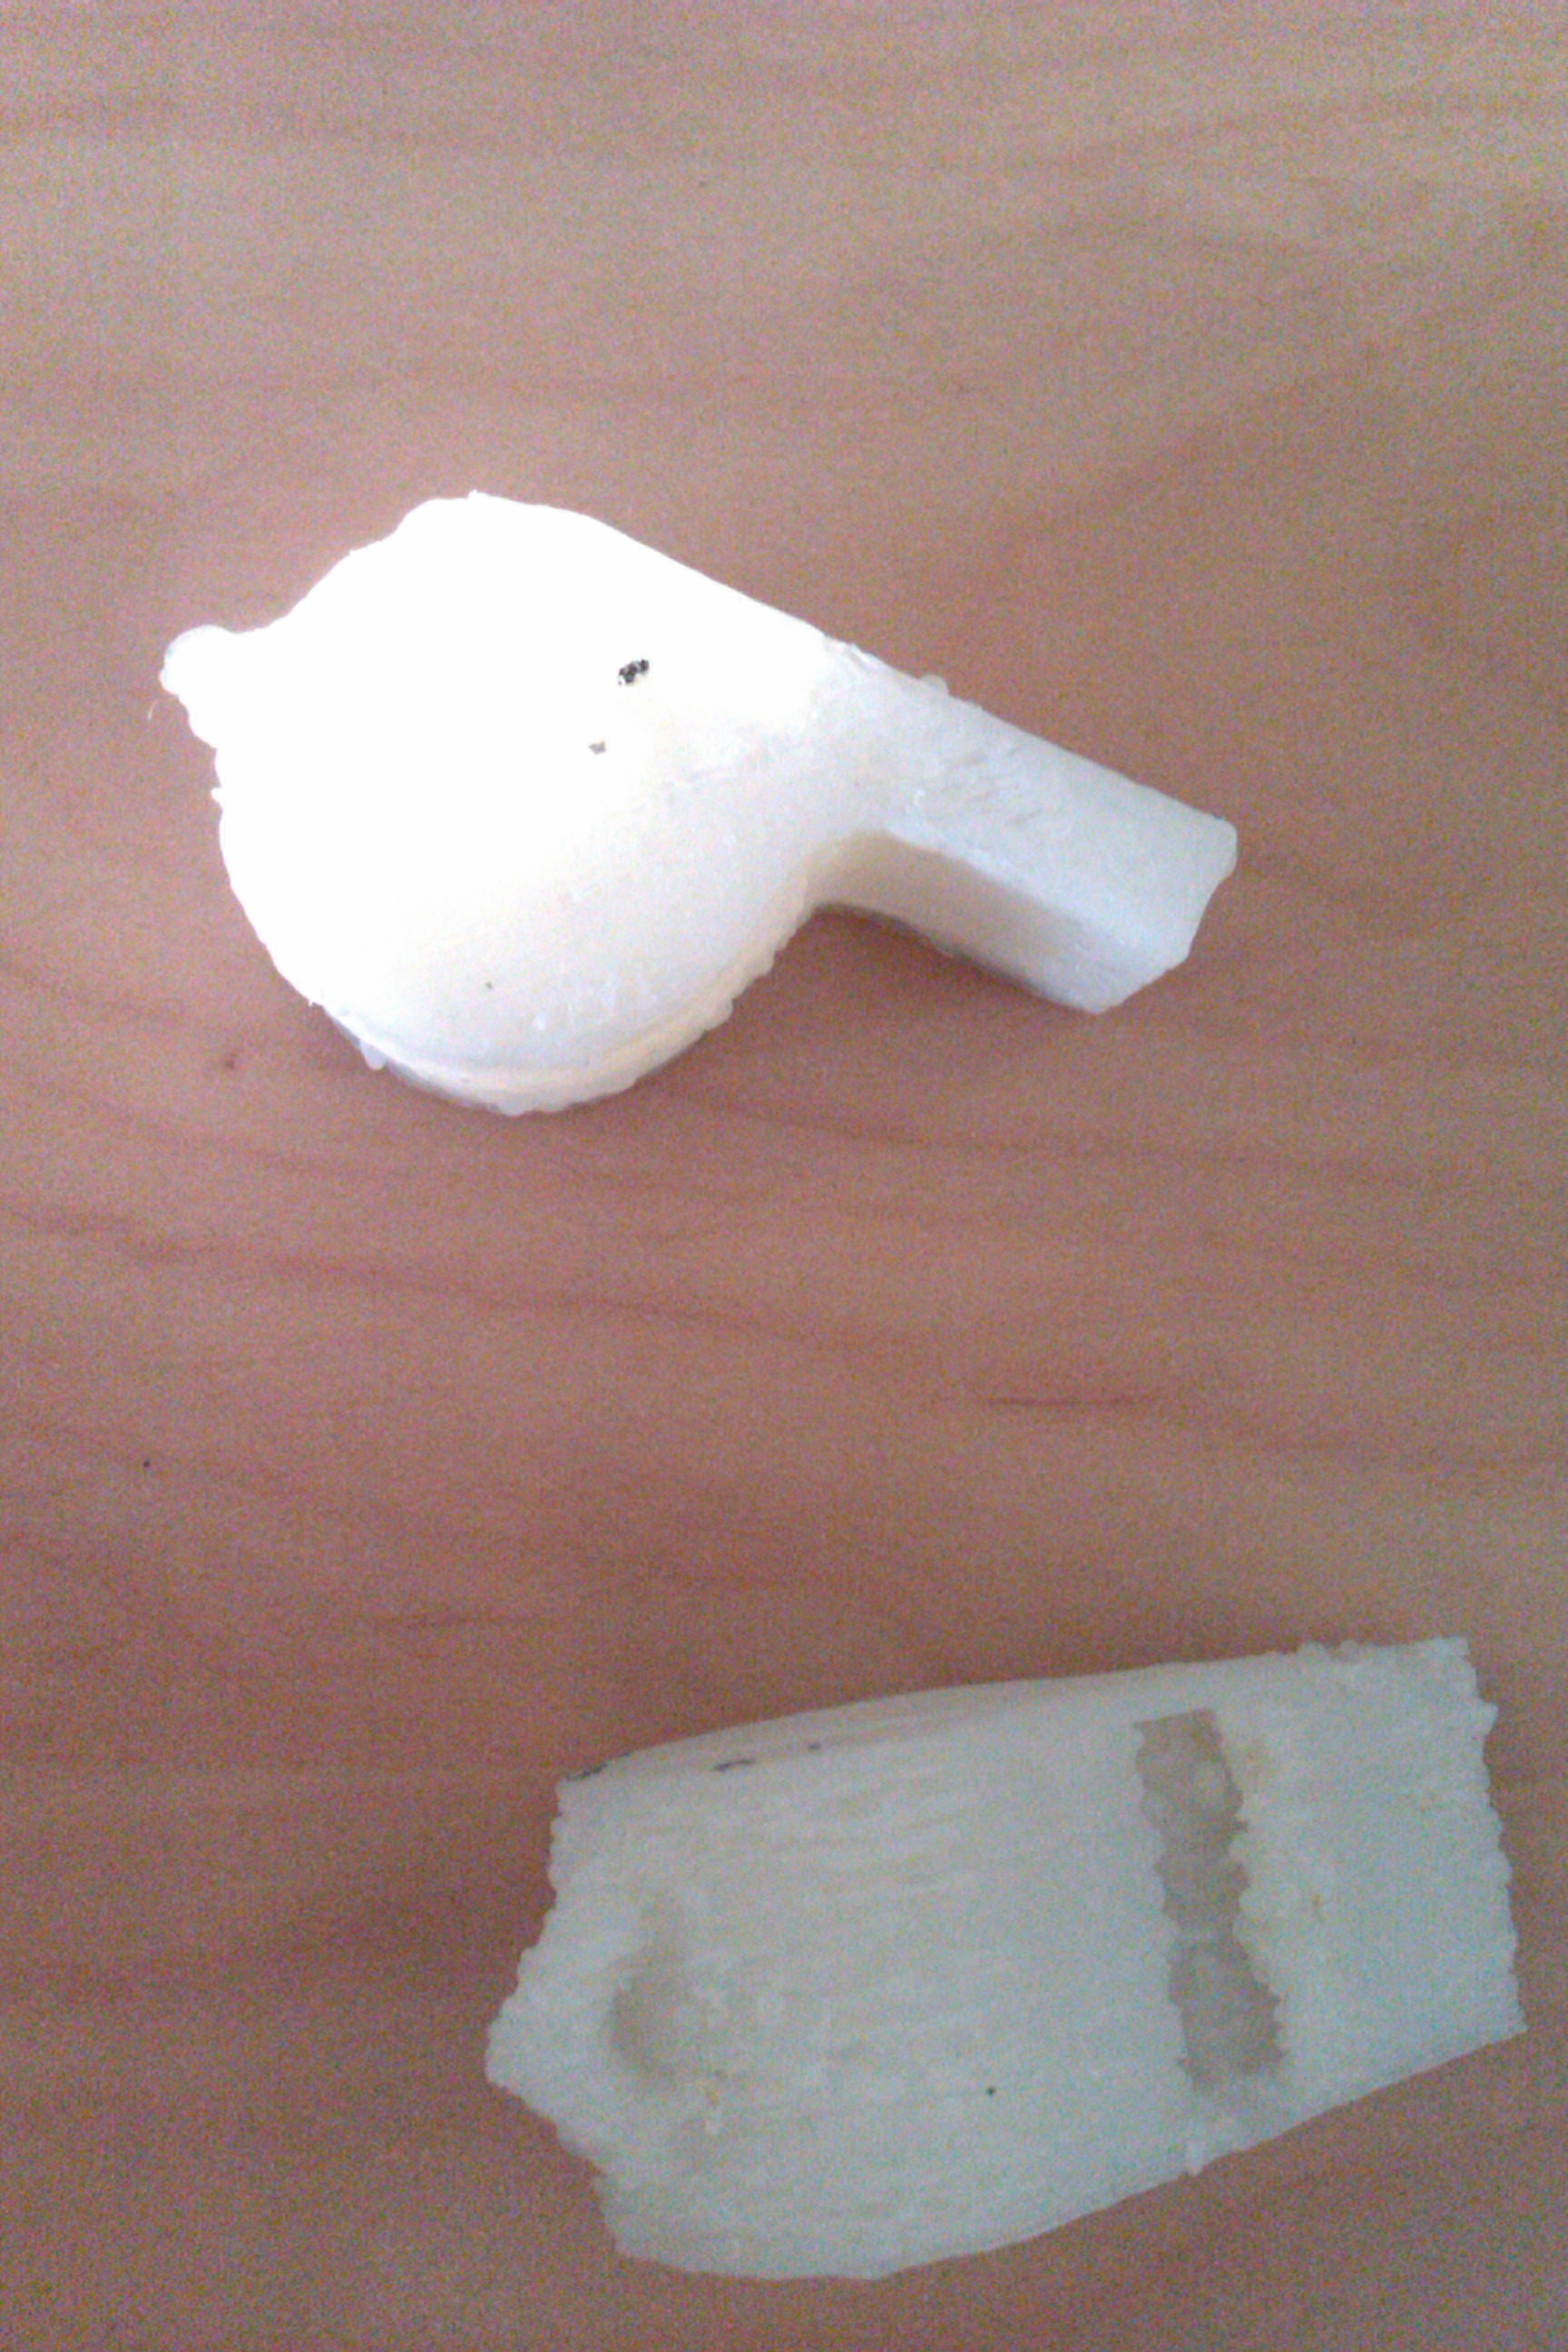
\includegraphics[scale=0.085]{IMAG0412.jpg}
}

\section{Afsluiting}
\frame{
  \frametitle{Afsluiting}
  Zijn er nog vragen?
}

\end{document}
